% L22rpo.tex
% $Author$ $Date$

% \section{\Rpo s}
% \label{sec:rpos}
% Predrag created file              nov  2 2006

The \rpo s satisfy the condition $u(x+\shift,\period{}) = u(x,0)$,
where $\period{}$ is the period and $\shift$ the phase shift of \rpo .
We have limited our search to orbits with $\period{} < 200$ and found
over 250 prime orbits with $\shift > 0$.  Each \rpo\ with phase shift
$\shift \neq 0$ has a reflection symmetric partner
$u(x) \to -u(-x)$ with phase shift $-\shift$.  We have also found over
50 \po s, all of which possessing the symmetry $u(x,\period{}/2) =
{\bf R} u(x,0) = -u(-x,0)$ discussed in \refSect{sec:KSePO}.

The search has not been exhaustive, and there are likely to be more
orbits with $\period{} < 200$, especially with longer periods.
However, the orbits we have found provide a representative sample of
typical periodic and \rpo s and approximate well the chaotic
attractor (since they were located using seeds obtained from close
returns within the chaotic dynamics).

\begin{figure}[t]
\begin{center}
(a) 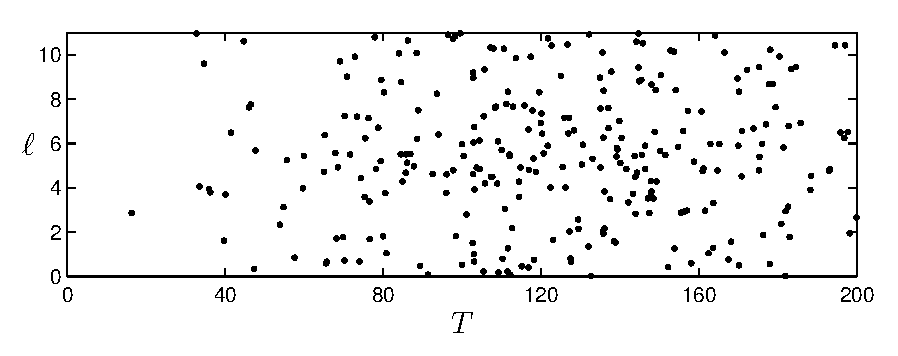
\includegraphics[width=0.7\textwidth]{figs/ks22_rpos_Tdelta.eps}
\\
(b) 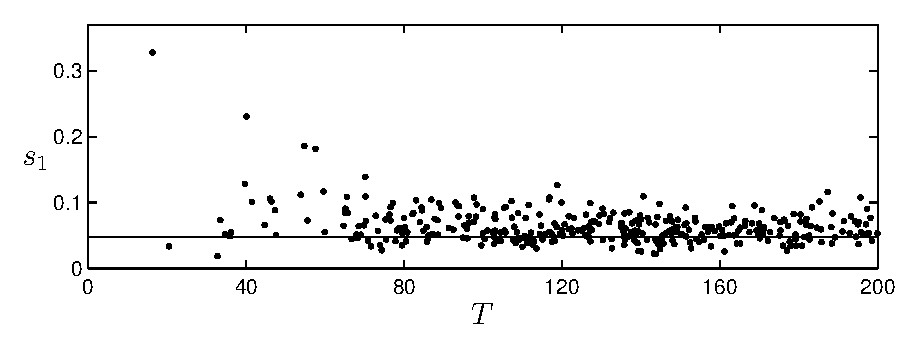
\includegraphics[width=0.7\textwidth]{figs/ks22_rpos_lyap.eps}
\end{center}
\caption{
(a) \Rpo s of \KSe\ with period $\period{}$ and shift
$\shift > 0$.
(b) The largest Floquet exponents \ref{FloqExp} of all \po s
and \rpo s.  The horizontal
line indicates the value 0.048 of the largest Lyapunov exponent
of the chaotic attractor.
} \label{f:ks22rposT}
\end{figure}

\refFig{f:ks22rposT} shows the \rpo s in the plane
$(\period{},\shift)$.  Not much is learned from such plot other than
that for longer periods the \rpo s are scattered over the
whole $(\period{},\shift)$.

The stability of the orbits is determined by their Floquet exponents,
defined as
\beq
\RLDedit{s_j} = \eigRe[j]/\period{} \,,
\ee{FloqExp}
where $\ExpaEig_j = e^{\eigRe[j] \pm i \eigIm[j]}$ are the
Floquet multipliers of $\jMps_p = g(\shift)J^T(a)$.
\PC{do not like notation $h_j$ for `Lyapunov exponent',
    I use $h$ for topological entropy }
\RLD{I've replaced $h_j$ with $s_j$.  Other options could be
$\lambda_j$, or $\sigma_j$, whichever you prefer.}


As could be expected from the calculation of the Lyapunov
exponents of the chaotic dynamics discussed in \refSect{sec:L22},
for all periodic and \rpo s we have found, only four Floquet
exponents are dynamically relevant, with the remaining ones being
very negative, indication strong contraction towards the 4-dimensional
manifold containing the chaotic attractor.  Out of the four
relevant exponents, two are equal to zero, corresponding to
time and space translational invariance of the orbits.  Of the
remaining two one is always positive, while the second one is either
positive or negative, indicating non-hyperbolicity of the
chaotic attractor through unstable dimension variability
[Ref.???\RLD{Maybe give reference to one of the classical papers on
UDV, for example, R. Abraham and S. Smale, Proc. Symp. Pure Math.
{\bf 14}, 5 (1970), or  S. P. Dawson, C. Grebogi, T. Sauer,
and J. A. Yorke, Phys. Rev. Lett. {\bf 73}, 1927 (1994)}].

The scatter of the % real parts of the
largest Floquet exponents
of periodic and \rpo s is shown in \reffig{f:ks22rposL}.
In this case a tendency of accumulation toward the largest
Lyapunov exponent 0.048 of the chaotic attractor
%\PC{guys, do you mind estimating the
%    Lyapunov exponent by a long-time numerical simulation? It is needed as
%    a thin horizontal line in \reffig{f:ks22rposL}}
can be noted.  This, however, is in part an artifact of initializing
the \rpo\ searches by near recurrences in
long-time \statesp\ trajectories.

Next we describe several types of \rpo s.

\subsection{Short \rpo s}

The small period \rpo s outline the
coarse structure of the chaotic attractor, while the longer period
\rpo s resolve the finer details of the dynamics
without significant modification of this structure.

The first five orbits with the shortest period we have found are
shown in \reffig{f:ks22rposShort}.  The shortest orbit with
$\period{} = 16.4$ is also the most unstable, with one positive
Floquet exponent equal 0.328.  The other short orbits are less
unstable, with the largest Floquet exponent, $s_1$, in the range
0.018 -- 0.073.

%The orbit with $\period{} = 20.5$ is exactly periodic due to a
%special symmetry it possesses (see \refsect{ssec:po}).
%\PC{ please refer to the exact equation for this symmetry. }

\begin{figure}[t]
\begin{center}
%\includegraphics[width=0.9\textwidth]{figs/ks22rposShort.eps}
\begin{tabular}{ccccc} (a) & (b) & (c) & (d) & (e)\\
$t$
\includegraphics[width=0.18\textwidth]{figs/ks22rpo016.3-02.86.eps}\hspace{-3ex} &
\includegraphics[width=0.18\textwidth]{figs/ks22rpo032.8-10.96.eps}\hspace{-3ex} &
\includegraphics[width=0.18\textwidth]{figs/ks22rpo033.5-04.04.eps}\hspace{-3ex} &
\includegraphics[width=0.18\textwidth]{figs/ks22rpo034.6-09.60.eps}\hspace{-3ex} &
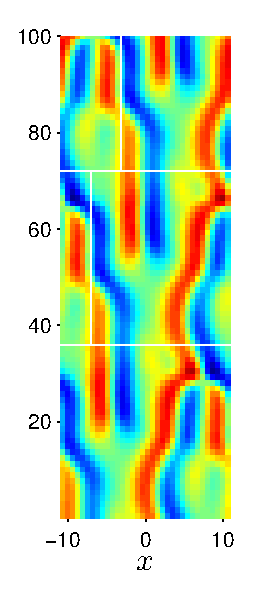
\includegraphics[width=0.18\textwidth]{figs/ks22rpo036.0-03.93.eps}
\end{tabular}
\end{center}
\caption{Short period \rpo s of \KSe\ with $L = 22$:
(a) $\period{} = 16.3$, $\shift = 2.86$;
(b) $\period{} = 32.8$, $\shift = 10.96$;
(c) $\period{} = 33.5$, $\shift = 4.04$;
(d) $\period{} = 34.6$, $\shift = 9.60$;
(e) $\period{} = 36.0$, $\shift = 3.93$.
Horizontal and vertical white lines indicate periodicity and phase
shift of the orbits, respectively.
}\label{f:ks22rposShort}
\end{figure}


    \RLD{
    \RLDedit{I've split the \reffig{f:ks22rposShort}
plots and put them in the tabular,
but I don't know how to place label $t$ to the left of the figures.
Please fix this if you know how.  Otherwise I can include $t$ in the
leftmost figure, but it will be a bit tricky since the aspect
ratio of this figure will be different from the others.
    }}
% \subsection{\Rpo s close to the unstable manifold of \EQV{2} }

We have found %\RLDedit{families of}
\rpo s which stay
%\RLDedit{arbitrarily long arbitrarily}
close to the unstable manifold of \EQV{2}.
%\RLD{To be precise, we haven't found families of arbitrarily
%long/close to cage orbits.  We can only speculate that such families
%exist, but what we've actually found was a handful of orbits that
%might belong to such families.}
As is illustrated in \reffig{f:ks22rposCage}, all such orbits have
shift $\shift \approx L/4$, similar to the shift of orbits within
the unstable manifold of \EQV{2}, which start at \EQV{2} and
converge to $\Shift_{L/4}$\EQV{2} (see \reffig{f:KS22E2man}). This
confirms that the `cage' of unstable manifolds of equilibria plays
an important role in organizing the chaotic dynamics of the \KS\
equation.

\begin{figure}[t]
\begin{center}
%\includegraphics[width=0.9\textwidth]{figs/ks22rposCage.eps}
\begin{tabular}{ccccc} (a) & (b) & (c) & (d) & (e)\\
$t$
\includegraphics[width=0.18\textwidth]{figs/ks22rpo047.6-05.68.eps}\hspace{-3ex} &
\includegraphics[width=0.18\textwidth]{figs/ks22rpo055.6-05.25.eps}\hspace{-3ex} &
\includegraphics[width=0.18\textwidth]{figs/ks22rpo059.9-05.44.eps}\hspace{-3ex} &
\includegraphics[width=0.18\textwidth]{figs/ks22rpo071.7-05.50.eps}\hspace{-3ex} &
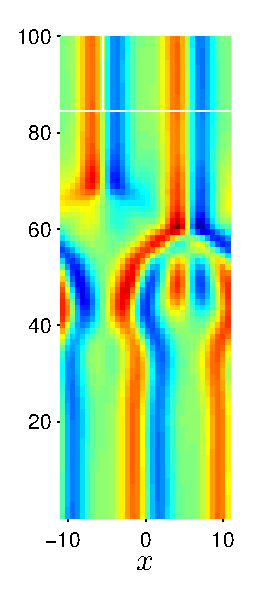
\includegraphics[width=0.18\textwidth]{figs/ks22rpo084.4-05.51.eps}
\end{tabular}
\end{center}
\caption{\Rpo s close to the unstable manifold of \EQV{2} equilibrium.
(a) $\period{} = 47.6$, $\shift = 5.68$;
(b) $\period{} = 55.6$, $\shift = 5.25$;
(c) $\period{} = 59.9$, $\shift = 5.44$;
(d) $\period{} = 71.7$, $\shift = 5.503$;
(e) $\period{} = 84.4$, $\shift = 5.513$.
Horizontal and vertical white lines indicate periodicity and
phase shift of the orbits, respectively. }\label{f:ks22rposCage}
\end{figure}


\subsection{Periodic Orbits} \label{ssec:po}
As discussed in \refSect{sec:KSePO}, a \rpo\ will be periodic, \ie,
$\shift = 0$, if it either {\bf (a)} lives within the antisymmetric
subspace $-u(-x,0) = u(x,0)$, or {\bf (b)} returns to its reflection
after half-period: $u(x,\period{}/2)=-u(-x,0)$.  The dynamics of
\KSe\ in the antisymmetric subspace and \po s with symmetry (a) have
been investigated
previously\rf{Christiansen:97,Lan:Thesis,LanCvi07}. The KS equation
with $L = 22$ does not have any periodic orbits of this type.

%The second symmetry implies that the \rpo\ is reflection-\-sym\-metric
%to itself after the time translation by half the period.

%So far we have found by trial and error 22 \po s
%(POs)
All the \po s we have found so far have symmetry (b).
%We have found over 50 \po s with $\period{} < 200$, with
%no guarantee that there might not exist many more of them.  The
%shortest such orbit is shown in \reffig{f:ks22rposShort}(b).
Some of the shortest \po s we have found are shown in
\reffig{f:ks22rposPO}.  Several \po s have been found by the same
method as used for locating \rpo s, while the other orbits have been
found by directly employing the symmetry condition:
\[ -u(-x+\shift,\period{}/2) = u(x,0)\,, \quad -L/2 < \shift \leq L/2\,.\]
In the Fourier space representation, this symmetry is expressed as
follows
\[
 -g(\shift)a^\ast(\period{}/2) = a(0)\,.
\]
This condition is used to find a \po\ with period $\period{}$
(compare it to the condition (\ref{eq:RPOcond}) for \rpo s).

%\PC{move most of this paragraph to flotsam.tex?}
%\RLDedit{We expect that the number of \po s with
%symmetry (b) and period $\period{}$ should be similar to the number
%of \rpo s with period $\period{}/2$.  The reason is that, provided
%the dynamics is equally mixing for all types of orbits,
%it should be equally possible to match $-u(-x+d,\period{}/2)$
%and $u(x,0)$, as it is to match $u(x+d,\period{})$ and $u(x,0)$,
%especially for larger $\period{}$.  So far, we have found 51 \po s
%with $\period{} < 200$ and 78 \rpo s with $\shift > 0$ and
%period $\period{} < 100$.}
%\RLD{What do you think about this paragraph?  Can we include it in
%the paper?}
% \RLD{ It looks like there
% might be many more \po s than I initially expected to find. In fact, I
% can even venture a guess that there are approximately as many \po s
% with symmetry (2) within $\period{} < 200$ as there are \rpo s within $\period{} <
% 100$. The reasoning is that it shouldn't be any harder to match
% $-u(-x+d,\period{}/2)$ and $u(x,0)$, than it is to match $u(x+d,\period{})$ and
% $u(x,0)$, provided the dynamics is equally mixing for all types of
% orbits.  If this is true, then the number of \po s with period smaller
% than $\period{}/2$ should be approximately equal to the number of \rpo s with
% period smaller than $\period{}$; the equality improving with increasing
% $\period{}$.
%     }

\begin{figure}[t]
\begin{center}
%\includegraphics[width=0.9\textwidth]{figs/ks22rposPO.eps}
\begin{tabular}{ccccc} (a) & (b) & (c) & (d) & (e)\\
$t$
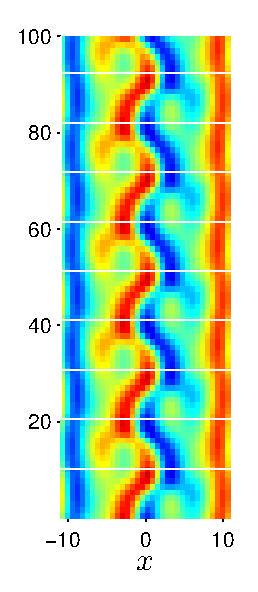
\includegraphics[width=0.18\textwidth]{figs/ks22rpo020.5-00.00.eps}\hspace{-3ex} &
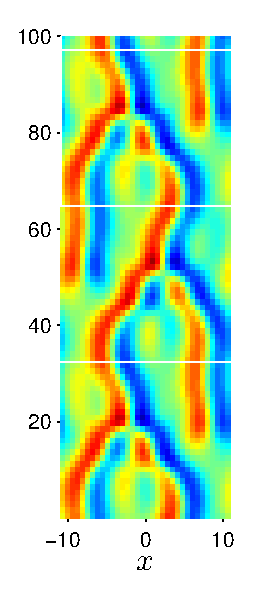
\includegraphics[width=0.18\textwidth]{figs/ks22rpo064.7-00.00.eps}\hspace{-3ex} &
\includegraphics[width=0.18\textwidth]{figs/ks22rpo066.8-00.00.eps}\hspace{-3ex} &
\includegraphics[width=0.18\textwidth]{figs/ks22rpo070.3-00.00.eps}\hspace{-3ex} &
\includegraphics[width=0.18\textwidth]{figs/ks22rpo077.2-00.00.eps}
\end{tabular}
\end{center}
\caption{\Po s of \KS\ equation with $L = 22$:
(a) $\period{} = 20.5$;
(b) $\period{} = 64.7$;
(a) $\period{} = 66.8$;
(b) $\period{} = 70.3$;
(c) $\period{} = 77.2$.} \label{f:ks22rposPO}
\end{figure}
